% CVPR 2022 Paper Template
% based on the CVPR template provided by Ming-Ming Cheng (https://github.com/MCG-NKU/CVPR_Template)
% modified and extended by Stefan Roth (stefan.roth@NOSPAMtu-darmstadt.de)

\documentclass[10pt,twocolumn,letterpaper]{article}

%%%%%%%%% PAPER TYPE  - PLEASE UPDATE FOR FINAL VERSION
\usepackage[review]{cvpr}      % To produce the REVIEW version
%\usepackage{cvpr}              % To produce the CAMERA-READY version
%\usepackage[pagenumbers]{cvpr} % To force page numbers, e.g. for an arXiv version

% Include other packages here, before hyperref.
\usepackage{graphicx}
\usepackage{amsmath}
\usepackage{amssymb}
\usepackage{booktabs}


% It is strongly recommended to use hyperref, especially for the review version.
% hyperref with option pagebackref eases the reviewers' job.
% Please disable hyperref *only* if you encounter grave issues, e.g. with the
% file validation for the camera-ready version.
%
% If you comment hyperref and then uncomment it, you should delete
% ReviewTempalte.aux before re-running LaTeX.
% (Or just hit 'q' on the first LaTeX run, let it finish, and you
%  should be clear).
\usepackage[pagebackref,breaklinks,colorlinks]{hyperref}


% Support for easy cross-referencing
\usepackage[capitalize]{cleveref}
\crefname{section}{Sec.}{Secs.}
\Crefname{section}{Section}{Sections}
\Crefname{table}{Table}{Tables}
\crefname{table}{Tab.}{Tabs.}


%%%%%%%%% PAPER ID  - PLEASE UPDATE
\def\cvprPaperID{MainQuest02} % *** Enter the CVPR Paper ID here
\def\confName{CVPR}
\def\confYear{2022}


\begin{document}

%%%%%%%%% TITLE - PLEASE UPDATE
\title{Autonomous driving assistance system with RetinaNet object detection}

\author{Youngmin Kim\\
AIFFEL\\
Modulabs\\
{\tt\small kym199907@gmail.com}
% For a paper whose authors are all at the same institution,
% omit the following lines up until the closing ``}''.
% Additional authors and addresses can be added with ``\and'',
% just like the second author.
% To save space, use either the email address or home page, not both
}
\maketitle

%%%%%%%%% ABSTRACT
\begin{abstract}
Object detection and decision-making are critical components of autonomous driving systems. This study aims to address the problem of determining "stop" or "go" decisions based on the detection of vehicles and pedestrians in real-time. Using the KITTI dataset, we developed a system that integrates RetinaNet, a state-of-the-art object detection model with a ResNet-50 backbone, to detect objects and determine actionable driving decisions.

The proposed system was trained for 20 epochs using a piecewise constant learning rate scheduler and evaluated on a validation dataset, achieving a classification accuracy of 0.8236. Additionally, the system demonstrated 100\% accuracy in stop/go evaluations using a sample test set of 10 images. The decision-making mechanism incorporated bounding box dimensions and pedestrian presence to determine driving actions, showcasing the system's applicability in real-world scenarios.

This research highlights the effectiveness of RetinaNet in handling imbalanced datasets and its integration into decision-making systems for autonomous driving. The study also identifies limitations, such as the need for evaluations under diverse environmental conditions, and outlines future research directions, including system optimization for real-time deployment. This work provides a foundational approach to object detection and decision-making for autonomous vehicles, contributing to safer and more efficient autonomous driving technologies.
\end{abstract}


%%%%%%%%% BODY TEXT
\section{Introduction}

Autonomous driving systems are transforming the transportation landscape by enhancing road safety, reducing human errors, and enabling efficient traffic management. A critical challenge in these systems is the ability to detect objects in real-time and make appropriate decisions based on the detected objects. Specifically, detecting vehicles and pedestrians and deciding whether to "stop" or "go" based on their presence is a fundamental problem for safe navigation.

Existing object detection models, such as SSD (Single Shot MultiBox Detector), have made significant strides in balancing speed and accuracy. However, SSD often struggles with detecting smaller objects or those in complex environments, leading to reduced reliability in critical scenarios. To address these limitations, we adopt RetinaNet, a state-of-the-art object detection model, known for its superior performance in handling class imbalance and detecting objects of varying sizes through the use of its focal loss function.

The KITTI dataset, a benchmark for autonomous driving research, was chosen for this study due to its comprehensive annotations for vehicles, pedestrians, and other relevant objects in real-world driving scenarios. This dataset provides a robust platform to evaluate the proposed system under realistic conditions.

In this work, we develop a system that utilizes RetinaNet with a ResNet50 backbone for object detection and implements custom logic to make "stop" or "go" decisions based on bounding box dimensions and the presence of pedestrians. Through extensive experimentation, we demonstrate that our system achieves high accuracy in both detection and decision-making, highlighting its applicability to real-world autonomous driving systems.

The remainder of this paper is organized as follows: Section 2 reviews related works, focusing on advancements in object detection and decision-making systems. Section 3 describes our methodology, including the dataset, model architecture, loss functions, and evaluation metrics. Section 4 presents the experimental results and analysis. Section 5 concludes the paper by summarizing key findings and discussing future directions. Acknowledgments and references are provided in Sections 6 and 7, respectively.

%------------------------------------------------------------------------
\section{Related Works}

\subsection{Object Detection Algorithms}
Object detection is a core component of autonomous driving systems. Over the years, several algorithms have been developed to improve detection accuracy and efficiency. Among the most notable are Faster R-CNN \cite{fasterrcnn}, SSD \cite{ssd}, and RetinaNet \cite{retinanet}. Faster R-CNN is known for its two-stage architecture, which provides high detection accuracy but at the cost of slower inference speeds. SSD, on the other hand, offers a single-stage approach, making it faster but less accurate in detecting small objects. RetinaNet addresses the class imbalance issue present in single-stage detectors by introducing the Focal Loss, enabling it to achieve a balance between speed and accuracy. For this study, RetinaNet was chosen due to its superior performance in detecting small objects and its efficiency in real-time scenarios.

\subsection{Datasets for Autonomous Driving}
Datasets play a pivotal role in training and evaluating object detection models. Commonly used datasets include COCO \cite{coco}, PASCAL VOC \cite{pascalvoc}, and KITTI \cite{kitti}. The KITTI dataset was selected for this study due to its focus on autonomous driving scenarios. It contains annotated images of vehicles, pedestrians, and other objects encountered in real-world driving conditions, making it particularly suitable for developing and testing autonomous driving systems.

\subsection{Integration of Detection and Decision}
While object detection has seen significant advancements, integrating detection results into actionable decisions, such as determining "stop" or "go," remains a challenge. Existing research often treats detection and decision-making as separate components, which can lead to inefficiencies and reduced performance in real-time applications. This study aims to bridge this gap by designing a system that directly utilizes detection outputs to make driving decisions, ensuring seamless integration and improved decision-making.

\subsection{Research Gaps and Contributions}
Despite advancements in object detection and autonomous driving research, several gaps remain:
\begin{itemize}
    \item Existing systems struggle to integrate detection and decision-making effectively.
    \item Many studies fail to address real-time performance requirements for stop/go decisions.
\end{itemize}
This study addresses these gaps by:
\begin{itemize}
    \item Leveraging the strengths of RetinaNet for high-accuracy object detection.
    \item Designing a decision-making system that integrates detection results to evaluate stop/go scenarios.
    \item Demonstrating the system's effectiveness using the KITTI dataset in real-world-like conditions.
\end{itemize}

%------------------------------------------------------------------------
\section{Method}

In this study, we utilize the KITTI dataset to evaluate the performance of our object detection framework. The methodology is outlined as follows:

\subsection{Dataset and Preprocessing}
The KITTI dataset, a widely used benchmark for autonomous driving tasks, was employed for training and evaluation. Images were resized and preprocessed to fit the input dimensions of the RetinaNet model.

\subsection{Model Architecture}
We adopted the RetinaNet model with a ResNet-50 backbone, pre-trained on the ImageNet dataset, for feature extraction. The model employs a feature pyramid network (FPN) for multi-scale feature representation and is designed to predict both object classes and bounding boxes.

\subsection{Training Configuration}
Training was conducted using TensorFlow 2.6.0 for 20 epochs. The learning rate schedule was defined using a piecewise constant decay method, with boundaries and values as follows:
\begin{itemize}
    \item \textbf{Boundaries:} [125, 250, 500, 240000, 360000]
    \item \textbf{Values:} [2.5e-06, 0.000625, 0.00125, 0.0025, 0.00025, 2.5e-05]
\end{itemize}

The learning rate schedule was implemented using the \texttt{PiecewiseConstantDecay} function. The optimizer used for training was stochastic gradient descent (SGD) with a momentum of 0.9.

\subsection{Loss Functions}
The total loss function consists of two components: a classification loss and a box regression loss.

\subsubsection{Classification Loss}
Focal loss was used to handle class imbalance during training. The focal loss is defined as:
\begin{equation}
\text{Focal Loss} = -\alpha (1 - p_t)^\gamma \log(p_t)
\end{equation}
where $p_t$ is the predicted probability of the ground truth class, $\alpha$ is a weighting factor, and $\gamma$ is a focusing parameter.

\subsubsection{Box Regression Loss}
Smooth L1 loss was used to refine the bounding box predictions. This loss is defined as:
\begin{equation}
\text{Smooth L1 Loss} =
\begin{cases} 
0.5 \cdot (\text{difference})^2 & \text{if } |\text{difference}| < \delta, \\
|\text{difference}| - 0.5 & \text{otherwise},
\end{cases}
\end{equation}
where $\delta$ is a threshold parameter.

The classification and regression losses were calculated separately and combined for each training iteration.

\subsection{Metrics}
Performance was evaluated using the mean Average Precision (mAP) metric at different Intersection over Union (IoU) thresholds. This metric is commonly used in object detection tasks to quantify the localization and classification accuracy.


%------------------------------------------------------------------------
\section{Result}

The model was evaluated using a set of 10 images, consisting of 5 images for the "stop" condition and 5 images for the "go" condition. The evaluation criteria for determining "stop" and "go" were as follows:

\begin{itemize}
    \item \textbf{"stop" condition}: 
    A bounding box corresponding to a vehicle has a width or height greater than or equal to 300px, or if there is a pedestrian present in the image.
    \item \textbf{"go" condition}: 
    All other cases where the conditions for "stop" are not met.
\end{itemize}

The evaluation achieved perfect accuracy with all 10 images classified correctly. The model successfully identified 5 "stop" images and 5 "go" images, with no misclassifications, reflecting its effectiveness in correctly interpreting the given conditions.

In terms of overall model performance, the classification accuracy on the validation dataset was \textbf{0.8236}, indicating a strong ability to classify the images accurately. This performance suggests that the model is well-tuned for the task, demonstrating reliable results in both the evaluation of specific images and general classification accuracy.

\begin{figure}[h]
    \centering
    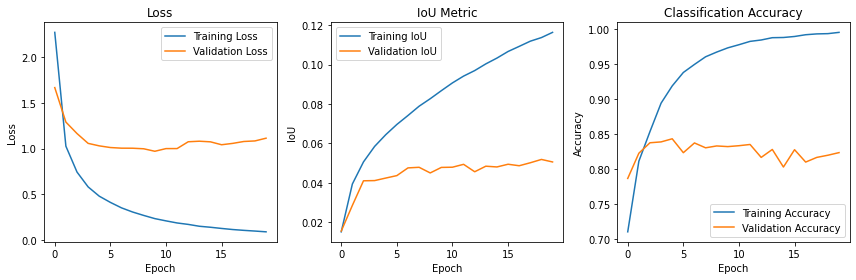
\includegraphics[width=0.8\linewidth]{graph.png}
    \caption{Losses and Metrics of the model across epochs.}
    \label{fig:graph}
\end{figure}

%------------------------------------------------------------------------
\section{Conclusion}

This study proposed a detection and decision-making system for autonomous driving, addressing the problem of determining “stop” or “go” decisions based on detected objects. Using the KITTI dataset and RetinaNet with ResNet-50 as the backbone, the system effectively integrated object detection results into actionable driving decisions. The system achieved a classification accuracy of 0.8236 on the validation dataset and demonstrated 100\% accuracy in stop/go evaluations using sample test images. These results highlight the robustness and applicability of the proposed system in autonomous driving scenarios.

The key contributions of this study include:
\begin{itemize}
    \item Employing RetinaNet for accurate and efficient object detection, particularly addressing the challenges posed by imbalanced datasets.
    \item Designing an integrated decision-making mechanism to evaluate stop/go scenarios, showcasing practical use cases in autonomous driving.
    \item Demonstrating the system's performance using the KITTI dataset in real-world-like conditions.
\end{itemize}

However, the study also has several limitations. The evaluations were conducted solely on the KITTI dataset, which may not generalize to other datasets or environments. Additionally, the system's performance under challenging conditions, such as adverse weather or low-light scenarios, was not explored. Furthermore, the study did not include real-time deployment tests, which are critical for practical autonomous driving applications.

Future research directions include expanding the system's evaluation to larger and more diverse datasets, improving robustness to various environmental conditions, and optimizing the model for real-time performance. Additionally, extending the decision-making capabilities to handle complex scenarios beyond binary stop/go decisions could further enhance the system's utility in autonomous driving.

In conclusion, this study provides a foundational approach to integrating object detection and decision-making in autonomous driving, demonstrating the feasibility and potential of such systems in real-world applications.

%------------------------------------------------------------------------
\section*{Acknowledgment}

This research was made possible by the KITTI dataset provided by the Karlsruhe Institute of Technology and Toyota Technological Institute at Chicago, which was instrumental for the development and evaluation of the proposed system. 

We would like to express our heartfelt gratitude to Modulabs' Aiffel program for providing the experimental environment, including both hardware and virtual platforms, which significantly facilitated our research. 

Special thanks to the Aiffel facilitators for their invaluable guidance and support throughout the study. Their insights and encouragement were critical in navigating challenges and ensuring the success of this research.

%------------------------------------------------------------------------
\begin{thebibliography}{99}

\bibitem{KITTI}
A. Geiger, P. Lenz, C. Stiller, and R. Urtasun, 
"Vision meets Robotics: The KITTI Dataset," 
\textit{International Journal of Robotics Research (IJRR)}, vol. 32, no. 11, pp. 1231–1237, 2013. 

\bibitem{RetinaNet}
T. Lin, P. Goyal, R. Girshick, K. He, and P. Dollár,
"Focal Loss for Dense Object Detection,"
in \textit{Proceedings of the IEEE International Conference on Computer Vision (ICCV)}, 2017, pp. 2980–2988.

\bibitem{SSD}
W. Liu, D. Anguelov, D. Erhan, C. Szegedy, S. Reed, C.-Y. Fu, and A. C. Berg,
"SSD: Single Shot MultiBox Detector,"
in \textit{Proceedings of the European Conference on Computer Vision (ECCV)}, 2016, pp. 21–37.

\bibitem{TensorFlow}
M. Abadi, P. Barham, J. Chen, Z. Chen, A. Davis, J. Dean, M. Devin, et al.,
"TensorFlow: A System for Large-Scale Machine Learning,"
in \textit{Proceedings of the 12th USENIX Conference on Operating Systems Design and Implementation (OSDI)}, 2016, pp. 265–283.

\bibitem{FocalLoss}
T. Lin, P. Goyal, R. Girshick, K. He, and P. Dollár,
"Focal Loss for Dense Object Detection,"
\textit{arXiv preprint arXiv:1708.02002}, 2017.

\end{thebibliography}

\end{document}
